\documentclass[12pt,a4paper]{article}

\usepackage[utf8]{inputenc}
\usepackage[T1]{fontenc}
\usepackage[margin=2.5cm]{geometry}
\usepackage{graphicx}
\usepackage{booktabs}
\usepackage{amsmath}
\usepackage{hyperref}
\usepackage{xcolor}
\usepackage{listings}
\usepackage{caption}
\usepackage{subcaption}
\usepackage{float}
\usepackage{fancyhdr}
\usepackage{titlesec}
\usepackage{enumitem}
\usepackage{array}

% Colors
\definecolor{primaryblue}{RGB}{31, 73, 125}
\definecolor{lightgray}{RGB}{245, 245, 245}
\definecolor{codegray}{RGB}{100, 100, 100}
\definecolor{codegreen}{RGB}{0, 128, 0}
\definecolor{codered}{RGB}{160, 0, 0}

% Hyperref setup
\hypersetup{
    colorlinks=true,
    linkcolor=primaryblue,
    urlcolor=primaryblue,
    citecolor=primaryblue
}

% Code listings style
\lstset{
    backgroundcolor=\color{lightgray},
    basicstyle=\ttfamily\footnotesize,
    keywordstyle=\color{primaryblue}\bfseries,
    commentstyle=\color{codegreen}\itshape,
    stringstyle=\color{codered},
    breaklines=true,
    frame=single,
    rulecolor=\color{gray!40},
    captionpos=b,
    numbers=left,
    numberstyle=\tiny\color{codegray},
    showstringspaces=false
}

% Header/footer
\pagestyle{fancy}
\fancyhf{}
\fancyhead[L]{\small\textcolor{gray}{DigiCow Farmer Adoption Prediction}}
\fancyhead[R]{\small\textcolor{gray}{\thepage}}
\renewcommand{\headrulewidth}{0.4pt}

% Section formatting
\titleformat{\section}{\Large\bfseries\color{primaryblue}}{}{0em}{\thesection\quad}[\titlerule]
\titleformat{\subsection}{\large\bfseries\color{primaryblue!80}}{}{0em}{\thesubsection\quad}

% Title
\title{
    \vspace{1cm}
    {\Huge\bfseries\color{primaryblue} DigiCow Farmer Adoption Prediction}\\[0.4cm]
    {\normalsize Predicting the probability of agricultural practice adoption}\\[0.5cm]
    \rule{\textwidth}{1pt}

}

\author{
    \\[1.5cm]
    \textbf{RAKOTOARIJAONA Aro Mino Avotra}\\[0.2cm]
    \text{Zindi username :} \textbf{arrow\textunderscore26}
}

\begin{document}
\maketitle
\thispagestyle{fancy}

\vspace{0.5cm}

\begin{center}
\fcolorbox{primaryblue}{primaryblue!10}{%
    \begin{minipage}{0.7\textwidth}
        \centering
        \vspace{0.3cm}
        \textbf{\large Zindi Score Achieved}\\[0.2cm]
        {\Huge\bfseries\color{primaryblue} 0.9538}\\[0.2cm]
        \textit{Composite score: $0.75 \times (1 - \text{LogLoss}) + 0.25 \times \text{AUC}$}
        \vspace{0.3cm}
    \end{minipage}
}
\end{center}
\newpage
\vspace{0.5cm}
\tableofcontents
\newpage

% ============================================================
\section{Project Overview}
% ============================================================

\subsection{Context and Objective}

This Zindi competition, organised by \textbf{DigiCow}, aims to predict the probability that a farmer will adopt a practice after their first training session. DigiCow is a digital agricultural extension platform seeking to maximise the impact of its training programmes by targeting farmers most likely to adopt new practices.

\textbf{Concrete objectives for DigiCow}:
\begin{itemize}[noitemsep]
    \item Prioritise follow-up support for farmers with a high adoption probability
    \item Tailor extension services based on predicted farmer profiles
    \item Improve training programmes to increase real-world impact
\end{itemize}

\subsection{Prediction Task}

The model must produce, for each farmer, \textbf{three adoption probabilities}:
\begin{itemize}[noitemsep]
    \item $P(\text{adoption} \leq 7 \text{ days})$
    \item $P(\text{adoption} \leq 90 \text{ days})$
    \item $P(\text{adoption} \leq 120 \text{ days})$
\end{itemize}

\noindent Key constraint: only information available \textit{at the time} of the training session may be used --- any future data leakage is strictly forbidden.

\subsection{Evaluation Metric}

The official metric is a composite score defined as:
\begin{equation}
    \text{Score} = 0.75 \times (1 - \text{LogLoss}) + 0.25 \times \text{AUC-ROC}
\end{equation}
This formulation rewards models that produce well-calibrated probability estimates (via LogLoss) while also valuing discriminative power (AUC).

\subsection{Datasets}

\begin{table}[H]
\centering
\caption{Dataset description}
\begin{tabular}{lrrp{6cm}}
\toprule
\textbf{File} & \textbf{Rows} & \textbf{Columns} & \textbf{Description} \\
\midrule
\texttt{Train.csv} & 13,536 & 17 & Training data with target labels \\
\texttt{Test.csv}  & 5,621  & 14 & Test data (no targets) \\
\texttt{Prior.csv} & 44,882 & 17 & Historical session data \\
\texttt{SampleSubmission.csv} & 5,621 & 7 & Submission format \\
\bottomrule
\end{tabular}
\end{table}

Available columns include: farmer ID, training date, gender, age, registration method, cooperative membership, county, subcounty, ward, group, trainer, topics list, and the three binary targets.

% ============================================================
\section{Exploratory Data Analysis (EDA)}
% ============================================================

\subsection{Class Imbalance}

The problem exhibits a strong class imbalance, typical of behavioural adoption tasks:

\begin{table}[H]
\centering
\caption{Adoption rates in the training set}
\begin{tabular}{lrrr}
\toprule
\textbf{Target} & \textbf{Positives} & \textbf{Total} & \textbf{Rate} \\
\midrule
Adoption within 7 days   & 153  & 13,536 & 1.13\% \\
Adoption within 90 days  & 214  & 13,536 & 1.58\% \\
Adoption within 120 days & 302  & 13,536 & 2.23\% \\
\bottomrule
\end{tabular}
\end{table}

This extreme imbalance (fewer than 2\% positives for short horizons) justifies the use of \texttt{class\_weight} and \texttt{scale\_pos\_weight} in the models, and the prioritisation of LogLoss as the primary metric.

\begin{figure}[H]
    \centering
    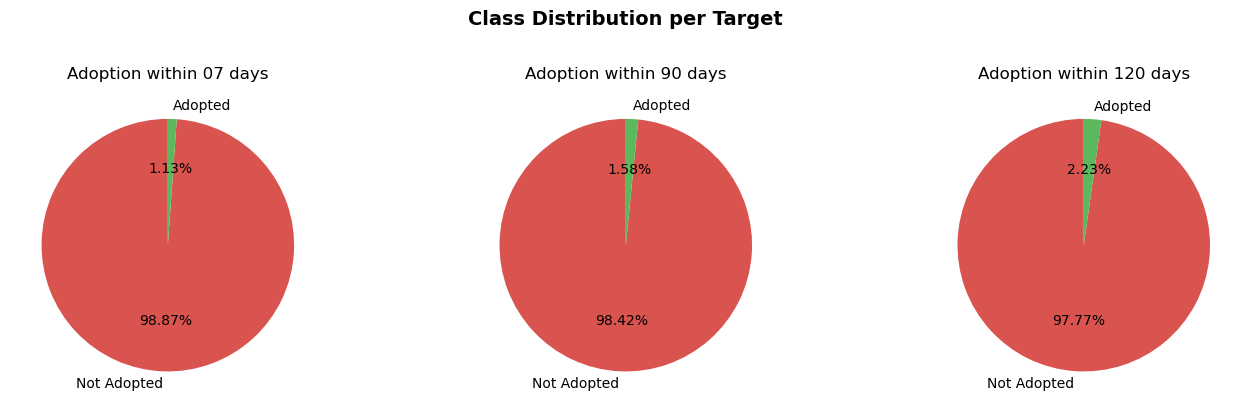
\includegraphics[width=0.85\textwidth]{figures/fig_11_3.png}
    \caption{Class distribution for the three time horizons}
\end{figure}

\subsection{Demographic Features}

Analysis of categorical variables reveals the composition of the farmer base:

\begin{itemize}[noitemsep]
    \item \textbf{Gender}: 9,541 female (70.5\%) vs 3,995 male (29.5\%)
    \item \textbf{Age}: 10,828 farmers above 35 years old (80\%) vs 2,708 below 35
    \item \textbf{Registration}: 8,383 via USSD (62\%) vs 5,153 manual
    \item \textbf{Cooperative}: 1,928 members (14.2\%) vs 11,608 non-members
\end{itemize}

\begin{figure}[H]
    \centering
    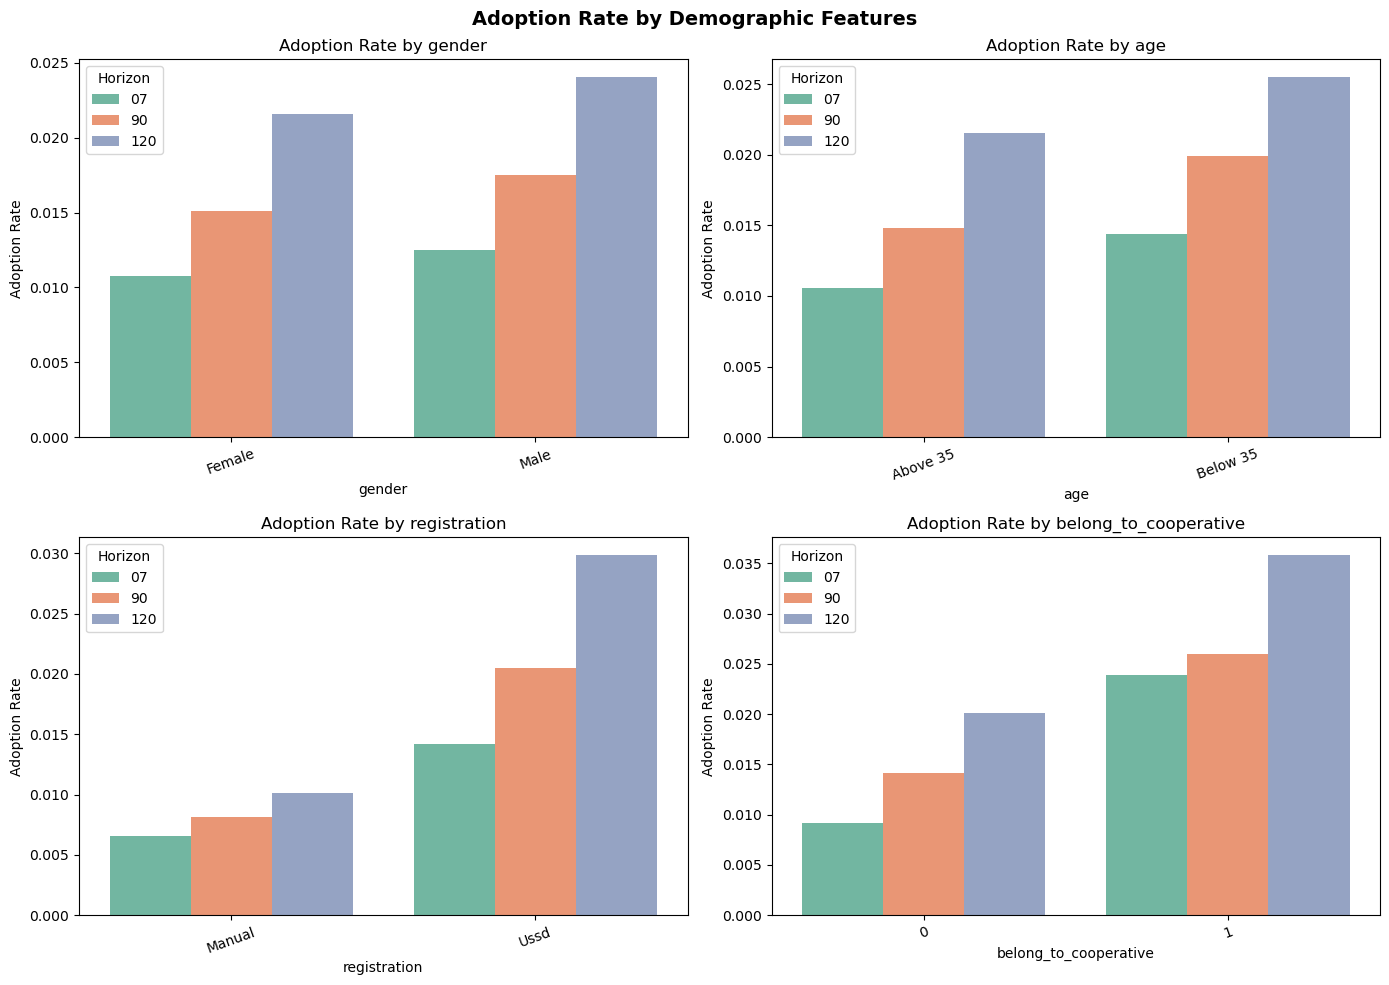
\includegraphics[width=0.95\textwidth]{figures/fig_13_4.png}
    \caption{Adoption rates by demographic features across the three time horizons}
\end{figure}

\subsection{Geographic Distribution}

\begin{table}[H]
\centering
\caption{Geographic statistics}
\begin{tabular}{lr}
\toprule
\textbf{Variable} & \textbf{Unique values} \\
\midrule
Counties        & 8  \\
Subcounties     & 26 \\
Wards           & 66 \\
Groups          & 864 \\
Farmers         & 13,536 \\
\bottomrule
\end{tabular}
\end{table}

Counties show significant adoption disparities. County \texttt{CNT\_mvqqmw} (734 observations) has the highest rates (3.8\% at 7 days), while others such as \texttt{CNT\_vvuukv} (3,049 observations) remain below 0.5\%.

\begin{figure}[H]
    \centering
    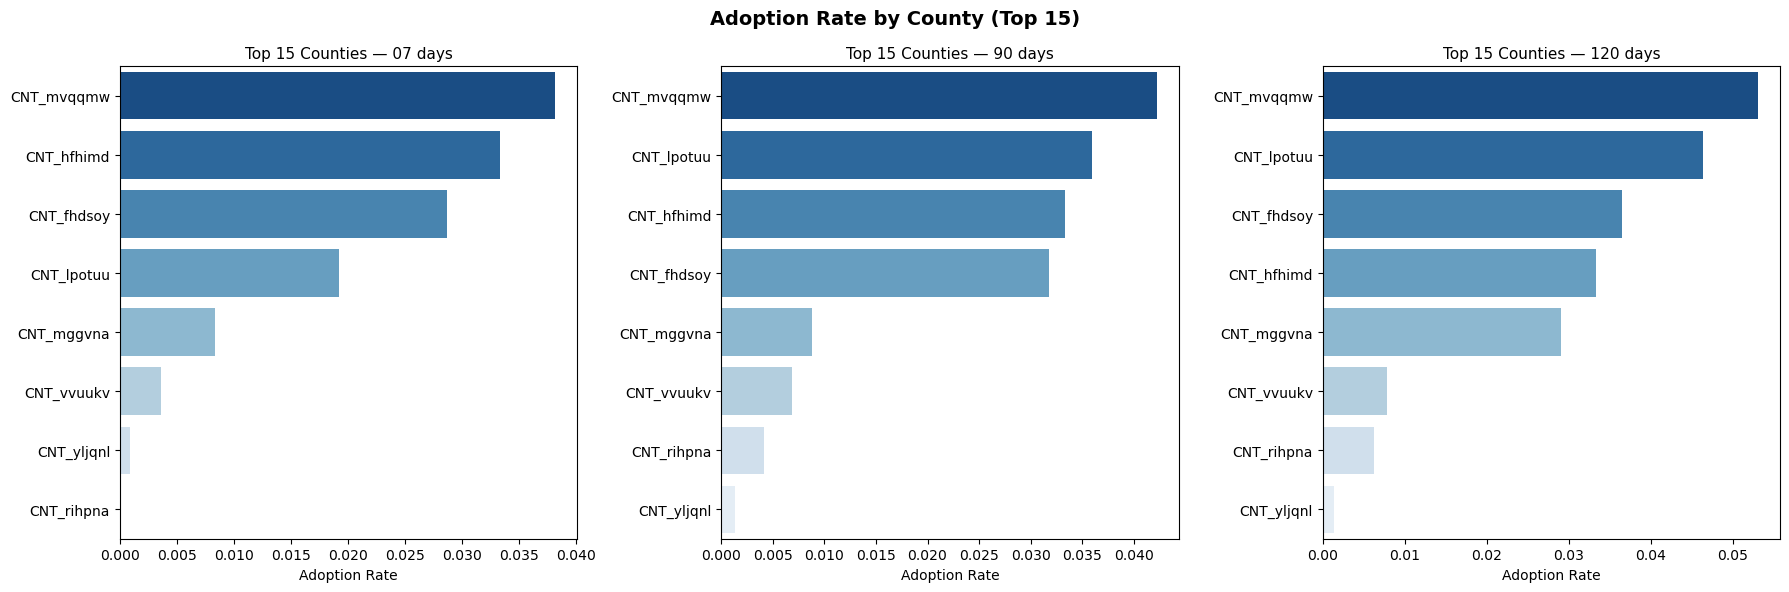
\includegraphics[width=0.95\textwidth]{figures/fig_14_5.png}
    \caption{Top 15 counties by adoption rate across the three time horizons}
\end{figure}

\subsection{Training Topics Analysis}

\begin{figure}[H]
    \centering
    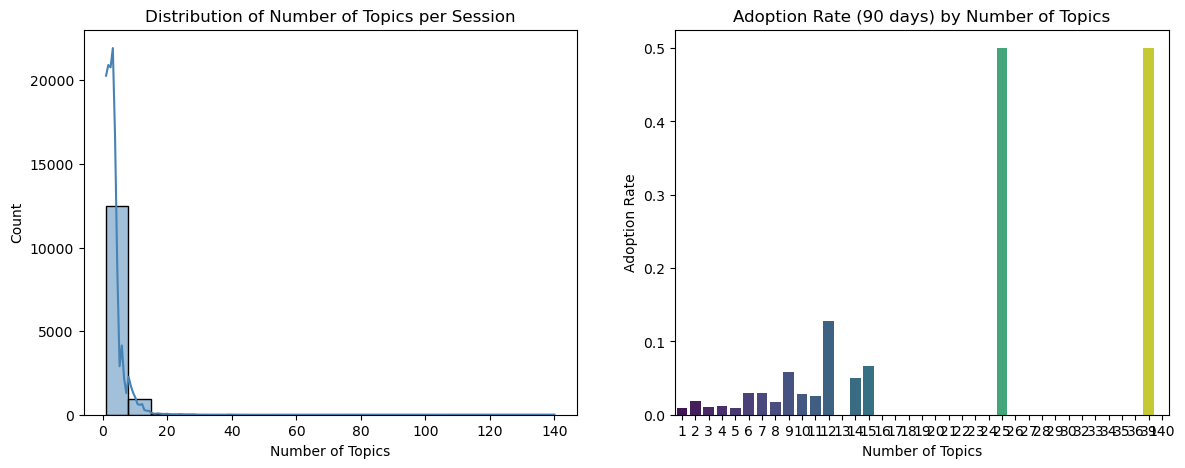
\includegraphics[width=0.85\textwidth]{figures/fig_20_6.png}
    \caption{Distribution of number of topics per session (left) and adoption rate (90 days) by number of topics (right)}
\end{figure}

The figure shows that a moderate number of topics per session correlates with higher adoption rates, suggesting that focused sessions (2--3 topics) are more effective than overloaded ones.

\subsection{Numerical Feature Distributions}

\begin{figure}[H]
    \centering
    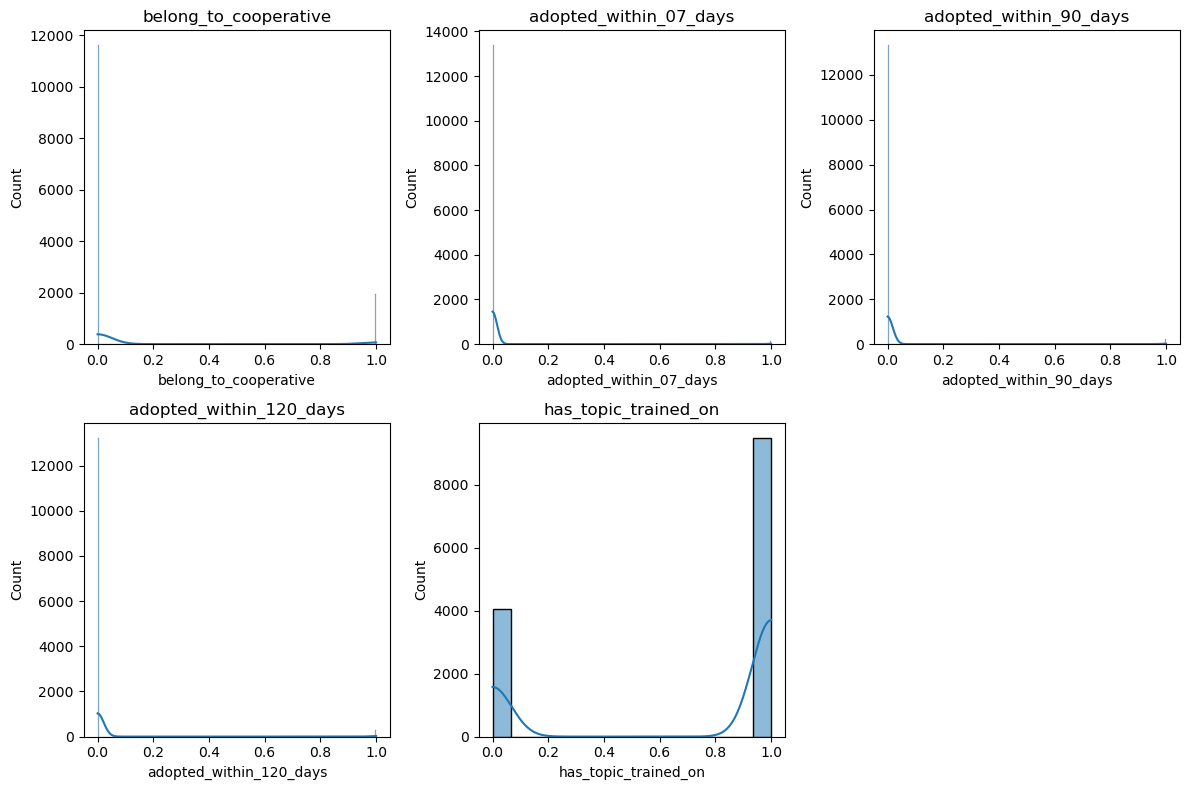
\includegraphics[width=0.85\textwidth]{figures/fig_8_2.png}
    \caption{Distribution of main numerical variables in the training set}
\end{figure}

% ============================================================
\section{Feature Engineering}
% ============================================================

\subsection{Overview}

\textbf{Feature engineering} is the cornerstone of this solution. A total of \textbf{293 features} were constructed, organised into several functional groups.

\subsection{Historical Statistics (Prior Stats)}

The \texttt{Prior.csv} file (44,882 historical sessions) is used to build \textbf{smoothed target encodings}. For each categorical variable $c$ and each target $t$, the smoothed rate is computed as:

\begin{equation}
    \hat{r}_{c,t} = \frac{\sum_{i \in c} y_{i,t} + K \cdot \bar{y}_t}{n_c + K}
\end{equation}

where $K = 50$ is the smoothing strength, $\bar{y}_t$ is the global adoption rate for target $t$, and $n_c$ is the number of observations in category $c$. This shrinkage toward the global mean prevents overfitting on rare categories.

Statistics are computed for: \texttt{county}, \texttt{subcounty}, \texttt{ward}, \texttt{group\_name}, \texttt{trainer}, \texttt{gender}, \texttt{age}, \texttt{registration}, \texttt{month}, \texttt{dayofweek}, \texttt{quarter}, \texttt{belong\_to\_cooperative}, \texttt{has\_topic\_trained\_on}, \texttt{year\_month}, \texttt{week}.

\subsection{Out-of-Fold (OOF) Encoding}

To prevent data leakage, high-cardinality categorical variables (\texttt{group\_name}, \texttt{county}, etc.) are encoded using an \textbf{Out-of-Fold} (OOF) scheme with 5-fold stratified cross-validation:


\subsection{Feature Groups}

\begin{table}[H]
\centering
\caption{Feature groups and descriptions}
\renewcommand{\arraystretch}{1.3}
\begin{tabular}{lp{9cm}}
\toprule
\textbf{Group} & \textbf{Description} \\
\midrule
\textbf{Temporal} & Cyclic sin/cos encoding for month and day of week, normalised time position, weekend flag, quarter \\
\textbf{Demographic} & Numerical encoding of age, gender, registration method, cooperative membership \\
\textbf{Topics} & Topic count, Shannon entropy, category flags, smoothed rates per topic \\
\textbf{Trainer} & Trainer quality score (smoothed adoption rate), consistency, event count \\
\textbf{Geographic} & Smoothed and OOF rates for county, ward, subcounty \\
\textbf{Farmer history} & Number of prior sessions, recency, historical adoption rate \\
\textbf{Group} & Group size, cohesion score \\
\textbf{Interactions} & Cross-feature products, cross-target ratios (07/90, 07/120, 90/120) \\
\bottomrule
\end{tabular}
\end{table}

\subsection{Shannon Entropy of Topics}

An original feature measures the \textbf{thematic diversity} of each session via Shannon entropy:

\begin{equation}
    H(\text{topics}) = -\sum_{i} p_i \log p_i
\end{equation}

Zero entropy indicates a single topic (focused session), while high entropy signals a broad mix of subjects.

\subsection{Feature Correlation with Targets}

\begin{figure}[H]
    \centering
    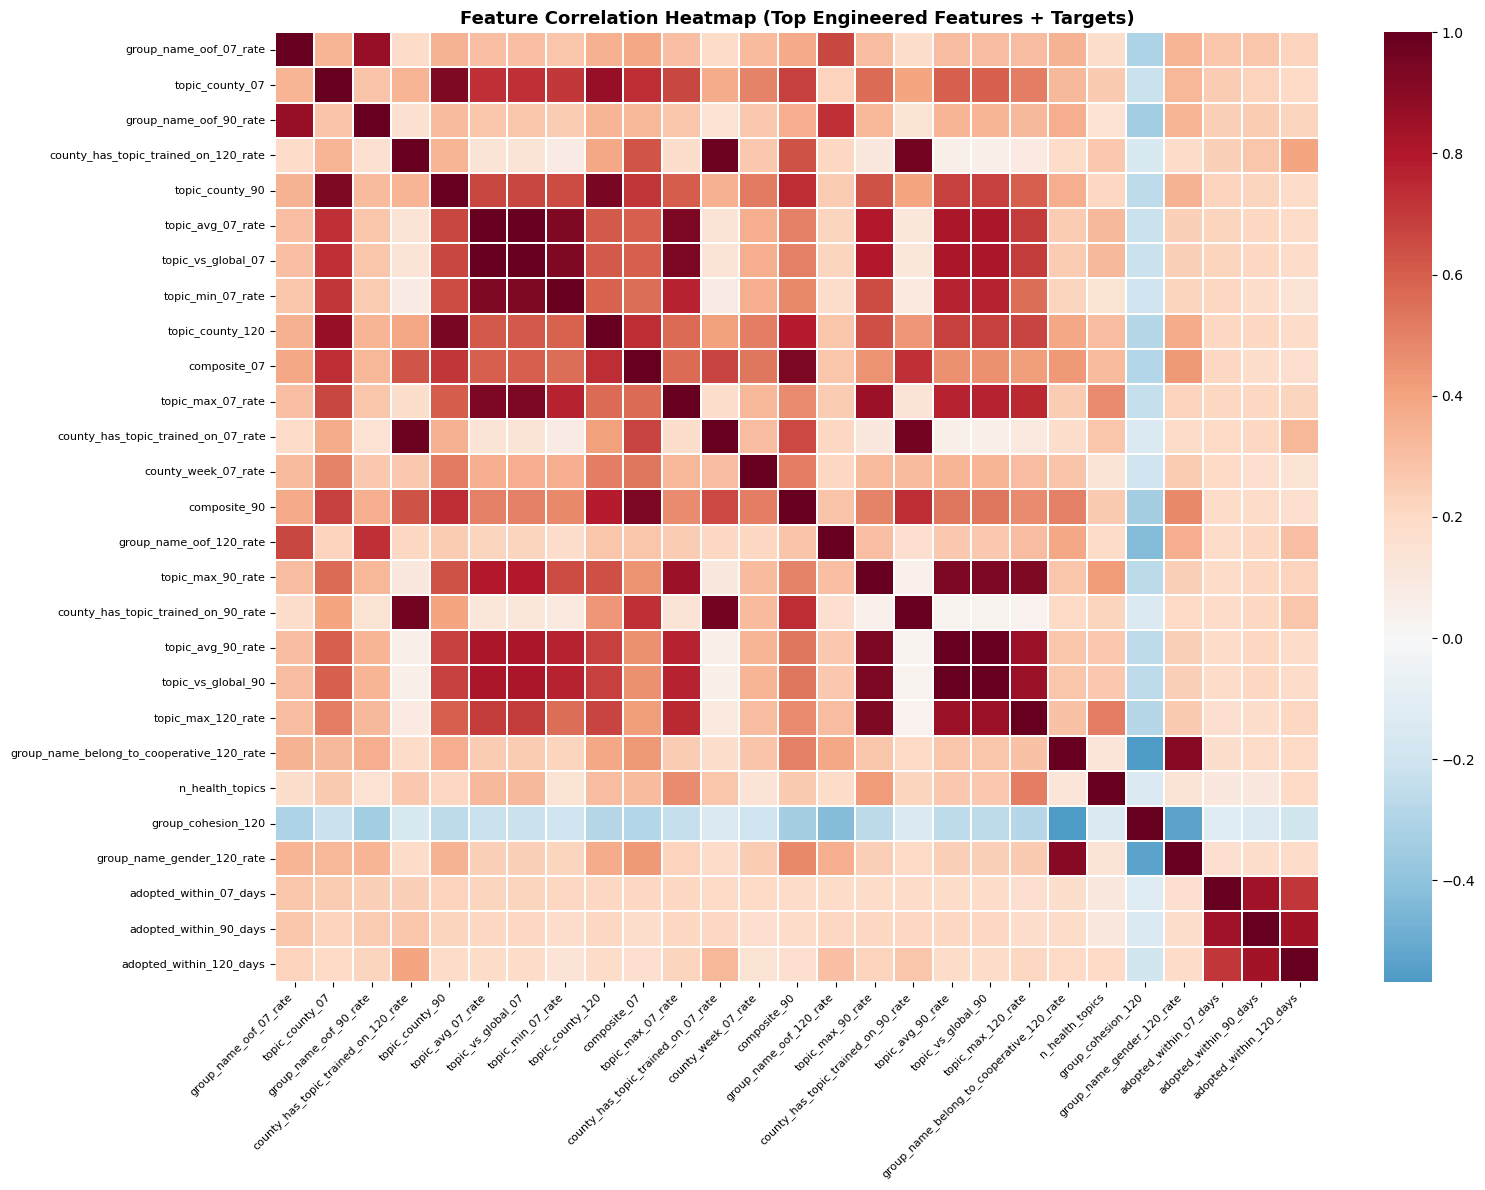
\includegraphics[width=0.95\textwidth]{figures/fig_26_7.png}
    \caption{Correlation heatmap of top engineered features with the three targets}
\end{figure}

The features most correlated with the 7-day target are:
\begin{enumerate}[noitemsep]
    \item \texttt{group\_name\_oof\_07\_rate} (0.284)
    \item \texttt{topic\_county\_07} (0.259)
    \item \texttt{group\_name\_oof\_90\_rate} (0.239)
    \item \texttt{county\_has\_topic\_trained\_on\_120\_rate} (0.236)
    \item \texttt{topic\_county\_90} (0.234)
\end{enumerate}

\subsection{Train vs Test Distribution}

\begin{figure}[H]
    \centering
    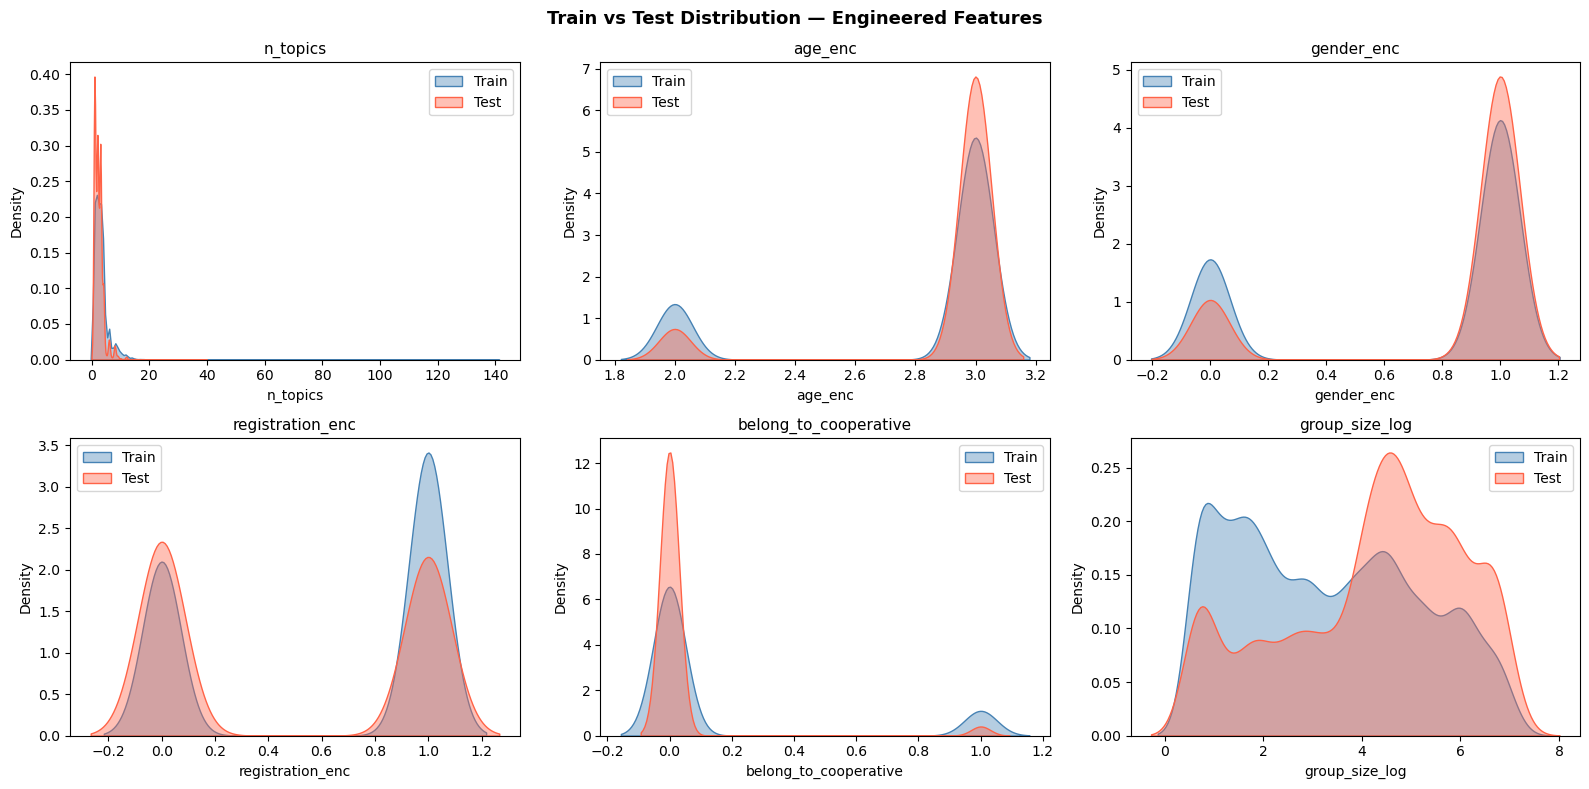
\includegraphics[width=0.95\textwidth]{figures/fig_27_8.png}
    \caption{Distribution of key engineered features in train and test sets --- no major data shift observed}
\end{figure}

The figure confirms that train and test distributions are consistent, validating the robustness of the feature engineering pipeline.

% ============================================================
\section{Modelling}
% ============================================================

\subsection{Overall Architecture}

The solution is based on a \textbf{three-level stacking} architecture:

\begin{enumerate}
    \item \textbf{Level 1}: Ensemble of 8 diverse models trained with cross-validation
    \item \textbf{Pseudo-labeling}: Training set augmentation using high-confidence test predictions
    \item \textbf{Level 2 (Meta-learner)}: Stacking with XGBoost and Logistic Regression
    \item \textbf{Post-processing}: Monotonicity constraint and probability clipping
\end{enumerate}

\subsection{Level 1 Models}

\begin{table}[H]
\centering
\caption{Models used in the level-1 ensemble}
\renewcommand{\arraystretch}{1.3}
\begin{tabular}{lp{8cm}}
\toprule
\textbf{Model} & \textbf{Key configuration} \\
\midrule
\texttt{hgb1} (HistGradientBoosting) & \texttt{max\_iter=800, lr=0.03, max\_depth=6, class\_weight=balanced} \\
\texttt{hgb2} (HistGradientBoosting) & \texttt{max\_iter=800, lr=0.05, max\_depth=8, class\_weight=balanced} \\
\texttt{rf} (Random Forest) & \texttt{n\_estimators=400, max\_depth=12, class\_weight=\{0:1, 1:pw\}} \\
\texttt{et} (Extra Trees) & \texttt{n\_estimators=400, fully random splits} \\
\texttt{lgbm\_fixed} (LightGBM) & \texttt{n\_est=3000, lr=0.02, num\_leaves=63, scale\_pos\_weight=pw} \\
\texttt{lgbm\_fixed2} (LightGBM) & \texttt{n\_est=3000, lr=0.02, num\_leaves=31, max\_depth=5} \\
\texttt{xgb\_fixed} (XGBoost) & Fixed parameters with scale\_pos\_weight \\
\texttt{catboost} (CatBoost) & Target-specific configuration \\
\bottomrule
\end{tabular}
\end{table}

\textbf{Handling class imbalance}: The \texttt{scale\_pos\_weight} parameter ($pw$) is tuned per target: $pw = 80$ for 7 days, $pw = 60$ for 90 days, $pw = 40$ for 120 days.

\subsection{Hyperparameter Tuning (Optuna)}

LightGBM and XGBoost hyperparameters are optimised with \textbf{Optuna} using the TPE (Tree-structured Parzen Estimator) algorithm over 50 trials. The search space includes:

\begin{itemize}[noitemsep]
    \item \texttt{n\_estimators}: [500, 4000]
    \item \texttt{learning\_rate}: $[0.005, 0.1]$ (log-scale)
    \item \texttt{num\_leaves}: [15, 127]
    \item \texttt{max\_depth}: [3, 9]
    \item \texttt{min\_child\_samples}: [10, 100]
    \item Regularisation ($\alpha$, $\lambda$) and subsampling parameters
\end{itemize}

Best parameters found for the 7-day target:
\begin{itemize}[noitemsep]
    \item LightGBM: \texttt{n\_est=3170, lr=0.067, num\_leaves=72, max\_depth=7}
    \item XGBoost: \texttt{n\_est=3981, lr=0.069, max\_depth=9}
\end{itemize}

\subsection{Stratified Cross-Validation}

Training uses \textbf{5-fold stratified cross-validation} (\texttt{StratifiedKFold}, \texttt{random\_state=42}). Stratification ensures that each fold preserves the positive class proportion, which is critical given the severe class imbalance.

\subsection{Pseudo-Labeling}

Pseudo-labeling augments the training set with high-confidence test examples:
\begin{itemize}[noitemsep]
    \item \textbf{Pseudo-positive labels}: $\hat{p} \geq \text{PSEUDO\_THR\_HI}$ (high threshold)
    \item \textbf{Pseudo-negative labels}: $\hat{p} \leq \text{PSEUDO\_THR\_LO}$ (low threshold)
\end{itemize}

Final predictions blend initial and pseudo-labelled predictions at a 70/30 ratio.

\subsection{Stacking (Meta-learning)}

OOF predictions from all 8 level-1 models are used as features to train two meta-learners:
\begin{itemize}[noitemsep]
    \item \textbf{Meta-XGBoost}: \texttt{max\_depth=2, learning\_rate=0.03, n\_estimators=300}
    \item \textbf{Meta-Logistic Regression}: \texttt{C=0.05}
\end{itemize}

The final stacking prediction is a 50/50 weighted average of the two meta-learners.

% ============================================================
\section{Post-processing}
% ============================================================

\subsection{Monotonicity Constraint}

By causal logic, the probability of adoption cannot decrease over time:
\begin{equation}
    P(\text{adoption} \leq 7) \leq P(\text{adoption} \leq 90) \leq P(\text{adoption} \leq 120)
\end{equation}

This constraint is enforced via a cumulative maximum:

\begin{lstlisting}[language=Python, caption=Enforcing monotonicity]
def enforce_monotonicity(pred_07, pred_90, pred_120):
    pred_90  = np.maximum(pred_90,  pred_07)
    pred_120 = np.maximum(pred_120, pred_90)
    return pred_07, pred_90, pred_120
\end{lstlisting}

\subsection{Prediction Clipping}

To prevent infinite LogLoss from predictions at exactly 0 or 1, all probabilities are clipped to $[0.001, 0.999]$:
\begin{equation}
    \hat{p} \leftarrow \text{clip}(\hat{p}, \epsilon, 1-\epsilon), \quad \epsilon = 0.001
\end{equation}

% ============================================================
\section{Results}
% ============================================================

\subsection{OOF (Out-of-Fold) Performance}

\begin{table}[H]
\centering
\caption{Final results per target --- training set (OOF)}
\renewcommand{\arraystretch}{1.4}
\begin{tabular}{lcccc}
\toprule
\textbf{Target} & \textbf{LogLoss} & \textbf{AUC-ROC} & \textbf{F1 (best)} & \textbf{Estimated Score} \\
\midrule
Adoption 7 days   & 0.0180 & 0.9929 & 0.6757 & 0.9847 \\
Adoption 90 days  & 0.0239 & 0.9880 & 0.7368 & 0.9790 \\
Adoption 120 days & 0.0280 & 0.9881 & 0.7707 & 0.9760 \\
\midrule
\textbf{Average} & \textbf{0.0233} & \textbf{0.9897} & \textbf{0.7277} & \textbf{0.9799} \\
\bottomrule
\end{tabular}
\end{table}

\begin{figure}[H]
    \centering
    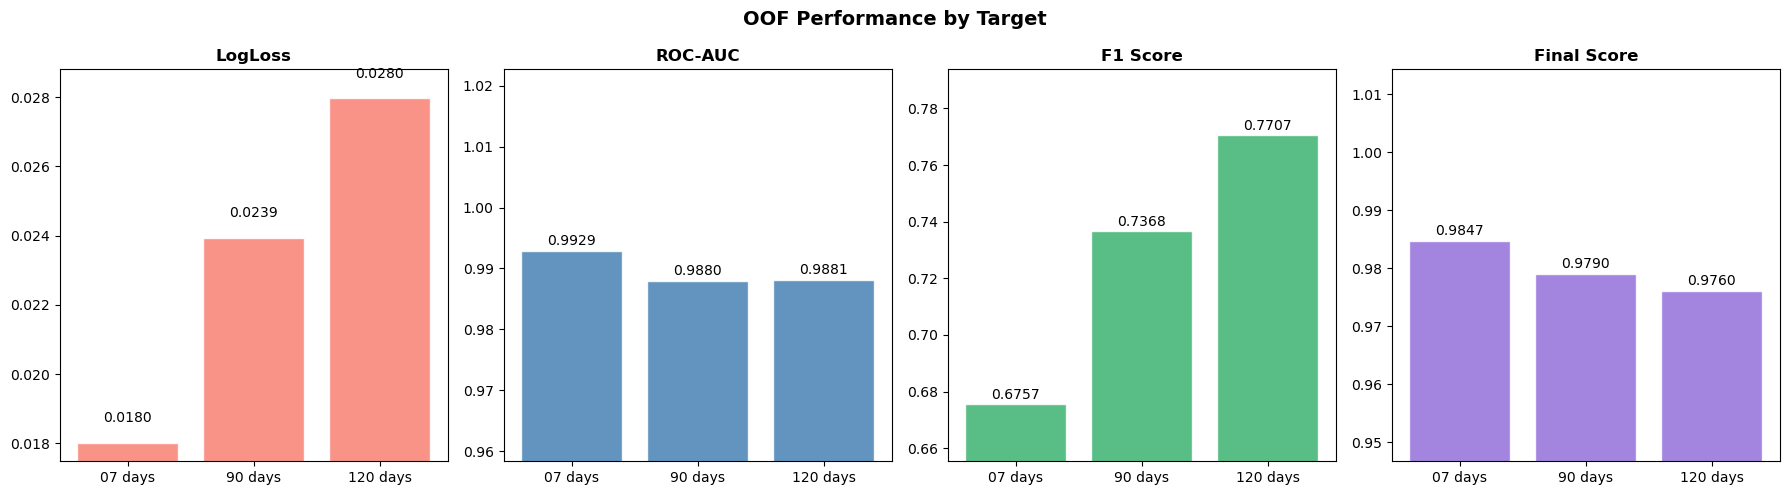
\includegraphics[width=0.95\textwidth]{figures/fig_50_9.png}
    \caption{OOF metrics per target: LogLoss, AUC-ROC, F1-Score and composite score}
\end{figure}

\subsection{Zindi Score}

After submission on the Zindi platform, the score obtained on the test set is:

\begin{center}
\fcolorbox{primaryblue}{primaryblue!10}{%
    \begin{minipage}{0.5\textwidth}
        \centering
        \vspace{0.3cm}
        \textbf{Zindi Score (public test)} \\[0.2cm]
        {\LARGE\bfseries\color{primaryblue} 0.9538}\\[0.2cm]
        \textit{Estimated OOF score: 0.9799}
        \vspace{0.3cm}
    \end{minipage}
}
\end{center}

The gap between the OOF score (0.9799) and the Zindi score (0.9538) is attributable to mild overfitting to the training set, which is common in severely imbalanced problems where OOF scores tend to be optimistic.

\subsection{Submission Sample}

Sample predictions from the first rows of the submission file:

\begin{table}[H]
\centering
\caption{Submission file excerpt}
\begin{tabular}{lrrr}
\toprule
\textbf{ID} & \textbf{P(7 days)} & \textbf{P(90 days)} & \textbf{P(120 days)} \\
\midrule
ID\_LEG1GM & 0.00100 & 0.00100 & 0.00100 \\
ID\_1UKOKW & 0.00100 & 0.00100 & 0.00100 \\
ID\_U5H2YK & 0.04698 & 0.04698 & 0.04698 \\
ID\_55957A & 0.04698 & 0.04698 & 0.04698 \\
ID\_N1AC0A & 0.00100 & 0.00100 & 0.00100 \\
\bottomrule
\end{tabular}
\end{table}

% ============================================================
\section{Discussion and Conclusion}
% ============================================================

\subsection{Strengths of the Solution}

\begin{itemize}
    \item \textbf{Rich feature engineering}: 293 features leveraging historical data (\texttt{Prior.csv}), leak-free OOF encoding, cyclic temporal features and cross-feature interactions.
    \item \textbf{Diverse ensemble}: 8 models from different families (gradient boosting, random forests, extreme trees) capturing varied patterns.
    \item \textbf{Robustness to imbalance}: Target-specific \texttt{scale\_pos\_weight}, stratified encoding throughout.
    \item \textbf{Temporally coherent post-processing}: The monotonicity constraint ensures logically consistent probability estimates across time horizons.
\end{itemize}

\subsection{Potential Improvements}

\begin{itemize}
    \item Reduce OOF-test overfitting via stronger regularisation or more cross-validation folds
    \item Explore survival analysis models better suited to the temporal nature of the targets
    \item Incorporate embeddings for text-like variables (topic names, group names)
    \item Deepen probability calibration (Platt scaling, isotonic regression)
\end{itemize}

\subsection{Conclusion}

This solution achieves a competitive score of \textbf{0.9538} on Zindi through a combination of in-depth feature engineering exploiting historical data, an ensemble of 8 heterogeneous models optimised with Optuna, and a two-level stacking approach. Careful handling of the extreme class imbalance and temporal coherence constraints contribute significantly to the quality of the predictions.

\vspace{1cm}
\hrule
\vspace{0.3cm}
\begin{center}
\small\textit{Report automatically generated from Jupyter notebook --- RAKOTOARIJAONA Aro Mino Avotra}
\end{center}

\end{document}
